\documentclass{article}
\usepackage[a4paper, top=25mm, bottom=40mm, 
   left=30mm, right=30mm]{geometry}
\usepackage[utf8]{inputenc}
\usepackage{standalone}
\usepackage{graphicx}
\usepackage{hyperref}
\usepackage{fancyhdr}
\usepackage{multirow}
\usepackage{tabularx}
\usepackage{blindtext}
\usepackage{array} % for defining a new column type
\usepackage{varwidth} %for the varwidth minipage environment
\usepackage[none]{hyphenat}
\usepackage[breakwords]{truncate}
\usepackage[noabbrev, capitalize]{cleveref}

\usepackage{dirtytalk}
\usepackage{enumitem}
\usepackage[utf8]{inputenc}
\usepackage{subfiles}
\usepackage{listings}
\usepackage{pstricks}

%%%%%%%%%%%%%%%%%%%%%%%%%%%%%%%%%%%%%%%%%%%%%%%%%%%%%%%%%%%%%
%   DOCUMENT DEFINITIONS
%%%%%%%%%%%%%%%%%%%%%%%%%%%%%%%%%%%%%%%%%%%%%%%%%%%%%%%%%%%%%
\def\doctitle{Documentation}
\def\teamname{SearchSECO}
\def\cpp{\cppnospace \space}
\def\cppnospace{\texttt{C++}}

\newcommand{\newpar}[1]{\paragraph{#1}\mbox{}\\}
\newcommand{\nocontentsline}[3]{}
\newcommand{\tocless}[2]{\bgroup\let\addcontentsline=\nocontentsline#1{#2}\egroup}

%%%%%%%%%%%%%%%%%%%%%%%%%%%%%%%%%%%%%%%%%%%%%%%%%%%%%%%%%%%%%
%   PREAMBLE
%%%%%%%%%%%%%%%%%%%%%%%%%%%%%%%%%%%%%%%%%%%%%%%%%%%%%%%%%%%%%
\setlength\parindent{0pt} % noindent
\graphicspath{ {Pictures/} }

\hypersetup{
    colorlinks=true,
    linkcolor=black,
    citecolor=black,
    filecolor=black,      
    urlcolor=blue,
    }

% HEADER
\addtolength{\headheight}{1.5cm} % make more space for the header
\pagestyle{fancyplain} % use fancy for all pages except chapter start
\lhead{
    \begin{tabular}{c l}
        \multirow{4}{*}{
\includegraphics[height=1.5cm]{secureseco-logo}} &\teamname \\[0.5ex]
        \cline{2-2}
        & \footnotesize\truncate{0.5\textwidth}{\doctitle} \\
        & \footnotesize \today
    \end{tabular}\vspace{1cm}}
\renewcommand{\headrulewidth}{0pt} % remove rule below header

% Tabularx settings
\newcolumntype{b}{X}
\newcolumntype{s}{>{\hsize=.33\hsize}X}


\begin{document}




%%%%%%%%%%%%%%%%%%%%%%%%%%%%%%%%%%%%%%%%%%%%%%%%%%%%%%%%%%%%%
%   DOCUMENT START
%%%%%%%%%%%%%%%%%%%%%%%%%%%%%%%%%%%%%%%%%%%%%%%%%%%%%%%%%%%%%
% ---------------------------------------------------------------------------------------------------------------------------------------------
% title page
\subfile{titlepage}

\restoregeometry

% general
\section{Introduction}
This is the full documentation of the \href{https://github.com/orgs/SecureSECO/teams/searchseco/repositories}{SearchSECO} system. It was created by a group of students from Utrecht University as Software Project in 2021 and then further developed after the conclusion of the project. We first give a brief overview of the system, after which all components are documented in detail individually. Following this, we discuss several interesting observations we made. Finally, we provide improvements that could be made in the future. Some parts of this documentation might be slightly outdated compared to the current version of the software\\




\clearpage
\tableofcontents
\clearpage

\section{Overview}

The system is built up out of several pieces of software, which can be divided in client-side and server-side. The server-side consists of the Database, its API and the Jobqueue. The client side consists of the Controller and its subcomponents (Crawler,Spider and Parser). The servers are manager by trusted parties. A client can be run by anyone on the world who want to contribute to the SearchSECO system. All components (including how they work together) are documented in detail below. 
\begin{figure}[h]
    \centering
    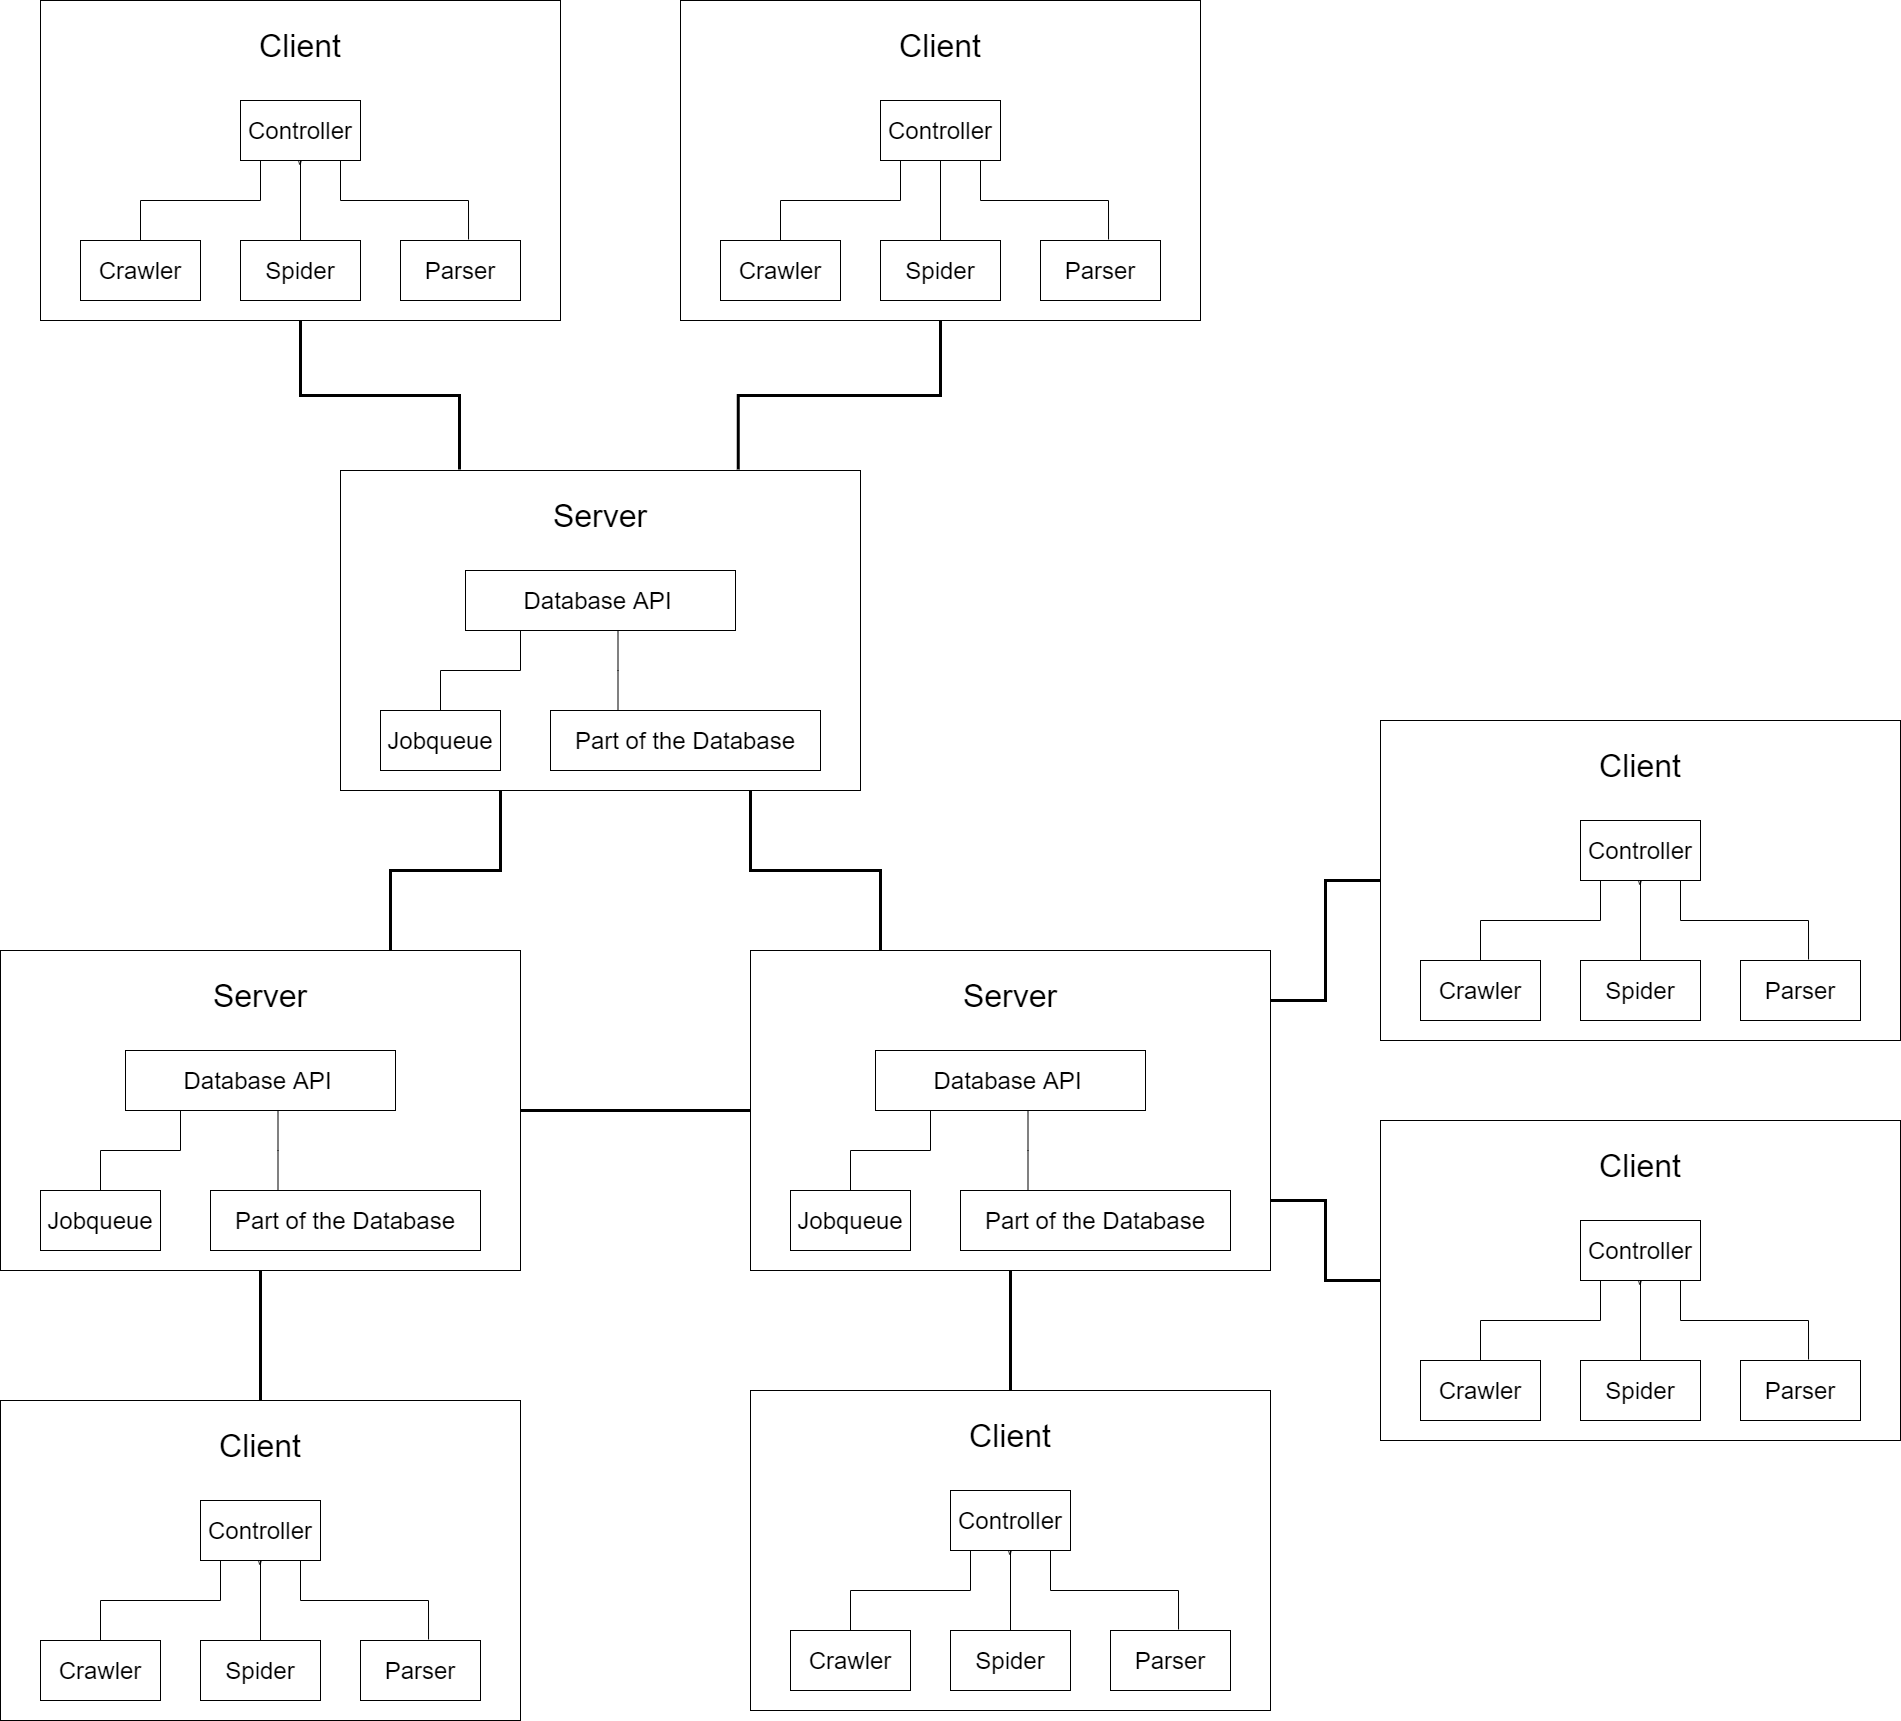
\includegraphics[width = \linewidth]{system-overview.png}
    \caption{An overview of the complete system}
    \label{fig:sysoverview}
\end{figure}
\clearpage

% client side
\subfile{"Components/Controller"}
\newpage
\subfile{"Components/Crawler"}
\subfile{"Components/Spider"}
\subfile{"Components/Parser"}

% server side
\subfile{"Components/Database"}

% improvements and such
\subfile{"Observations"}
\subfile{"FutureImprovements"}

% licenses
\subfile{"Licensing"}

\clearpage
\begin{thebibliography}{10}

\bibitem{VUDDY}
Kim, S., Woo, S., Lee, H. and Oh, H., 2017, May. Vuddy: A scalable approach for vulnerable code clone discovery. In 2017 IEEE Symposium on Security and Privacy (SP) (pp. 595-614). IEEE.
% You can add and cite as many new bibitems as you want; make sure to give them a unique and recognisable name.

\bibitem{github}
GitHub Inc. (\url{https://github.com}): a provider of Internet hosting for software development and version control using Git.

\bibitem{gitlab}
GitLab (\url{https://gitlab.com}): a web-based DevOps lifecycle tool that provides a Git-repository manager providing wiki, issue-tracking and continuous integration and deployment pipeline features, using an open-source license, developed by GitLab Inc.

\bibitem{shg}
Software Heritage Graph (\url{https://softwareheritage.org}): the largest existing public archive of software source code and accompanying development history. 

\bibitem{cassandra}
Apache Cassandra (\url{https://cassandra.apache.org/}): a free and open-source, distributed, wide-column store, NoSQL database management system designed to handle large amounts of data across many commodity servers, providing high availability with no single point of failure. Documentation can be found at  \url{https://cassandra.apache.org/doc/latest/}

\bibitem{srcML}
srcML: \url{https://www.srcml.org/}

\bibitem{ANTLR}
ANTLR: \url{https://www.antlr.org/}

\bibitem{curl}
libcurl (\url{https://curl.se/libcurl/}) is a free and easy-to-use client-side URL transfer library, supporting DICT, FILE, FTP, FTPS, GOPHER, GOPHERS, HTTP, HTTPS, IMAP, IMAPS, LDAP, LDAPS, MQTT, POP3, POP3S, RTMP, RTMPS, RTSP, SCP, SFTP, SMB, SMBS, SMTP, SMTPS, TELNET and TFTP.

\bibitem{loguru}
Loguru: \url{https://github.com/emilk/loguru}

\bibitem{boost}
Boost: \url{https://www.boost.org/}

\bibitem{code_clones_1}
Svajlenko, J., Islam, J.F., Keivanloo, I., Roy, C.K. and Mia, M.M., 2014, September. Towards a big data curated benchmark of inter-project code clones. In 2014 IEEE International Conference on Software Maintenance and Evolution (pp. 476-480). IEEE.

\bibitem{code_clones_2}
Farhadi, M.R., Fung, B.C., Charland, P. and Debbabi, M., 2014, June. Binclone: Detecting code clones in malware. In 2014 Eighth International Conference on Software Security and Reliability (SERE) (pp. 78-87). IEEE.

\end{thebibliography}

\clearpage
\section*{Appendix A: UML Diagrams}
This appendix contains the UML diagrams for the system. Some of these can be partially outdated or incomplete.
\begin{figure}[h]
    \centering
    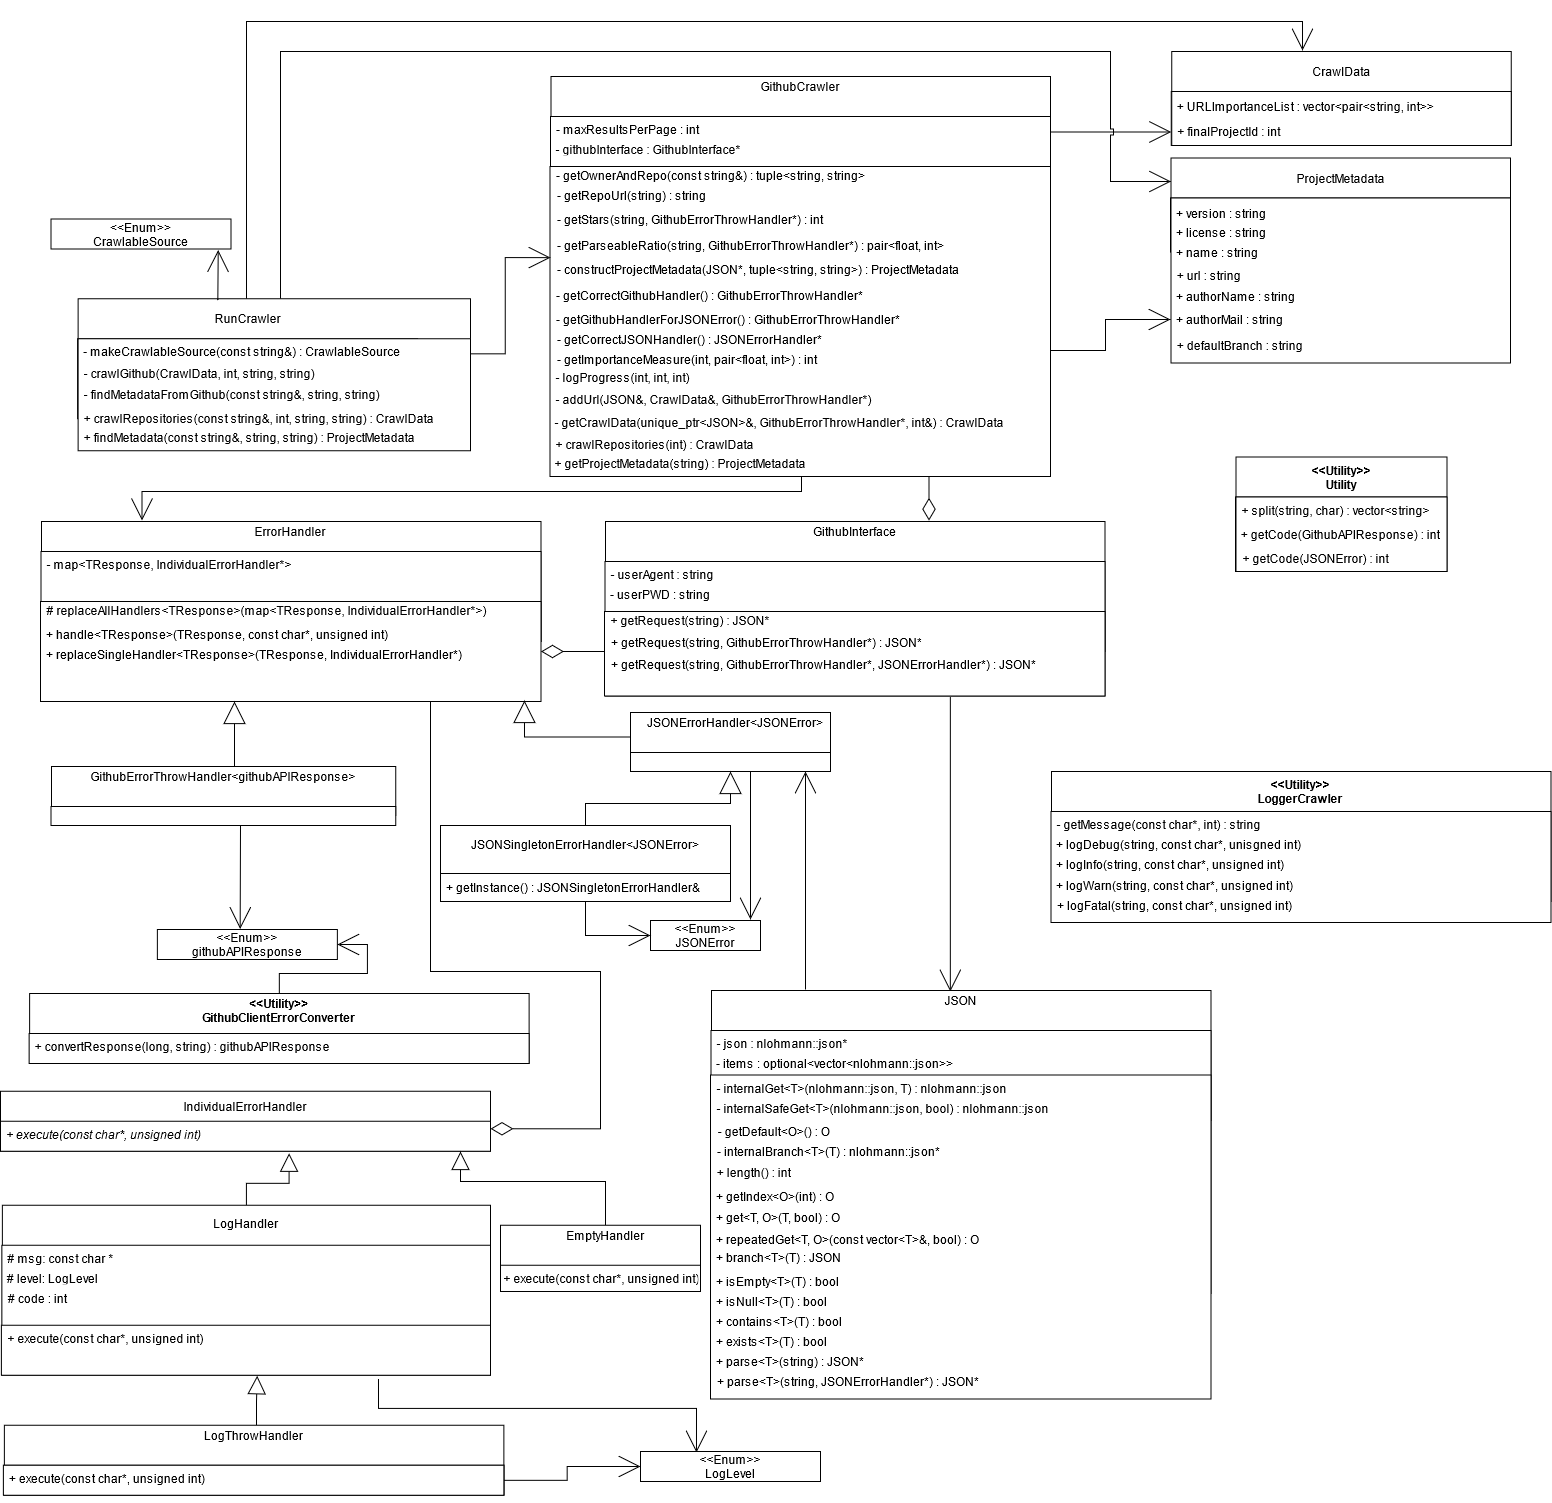
\includegraphics[width = \linewidth]{CrawlerUML.png}
    \caption{Crawler UML class diagram}
    \label{fig:umlcrawler}
\end{figure}

\begin{figure}
    \centering
    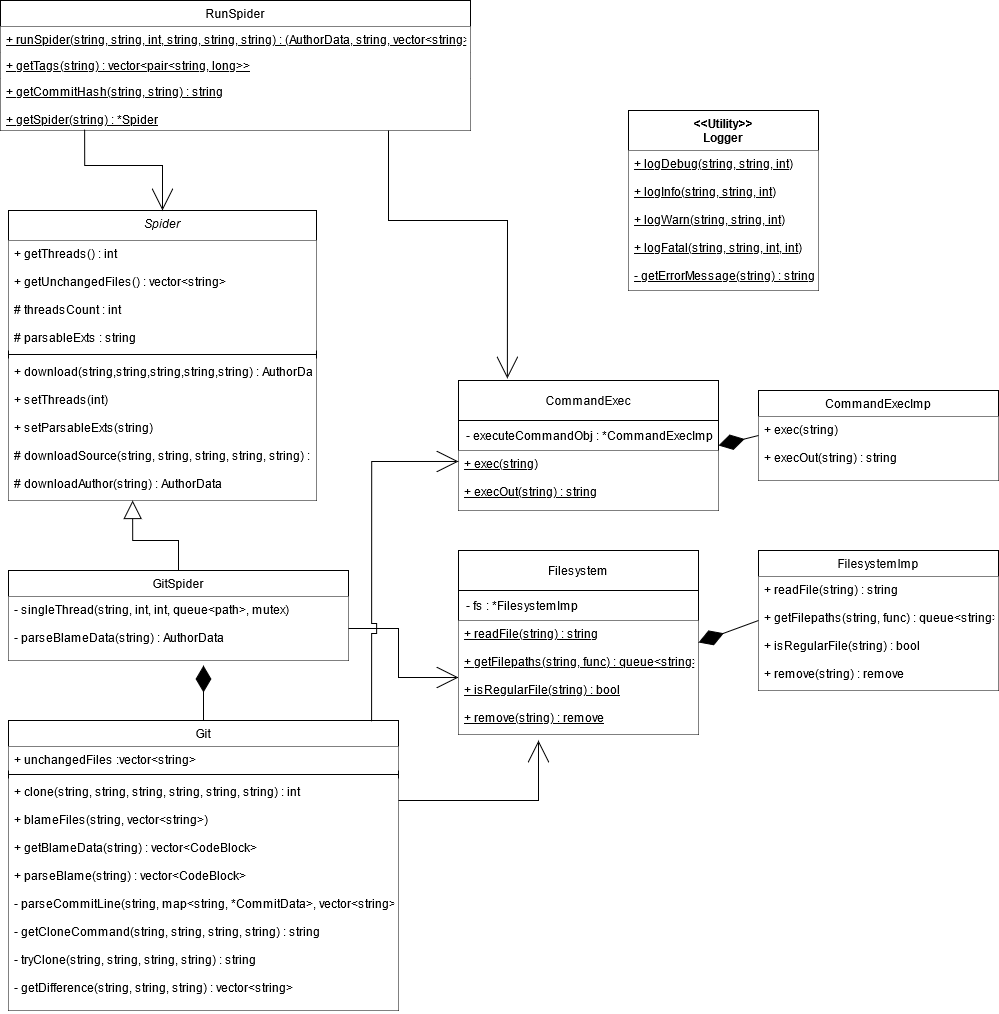
\includegraphics[width = \linewidth]{SpiderUML.png}
    \caption{Spider UML class diagram}
    \label{fig:umlspider}
\end{figure}

\begin{figure}
    \centering
    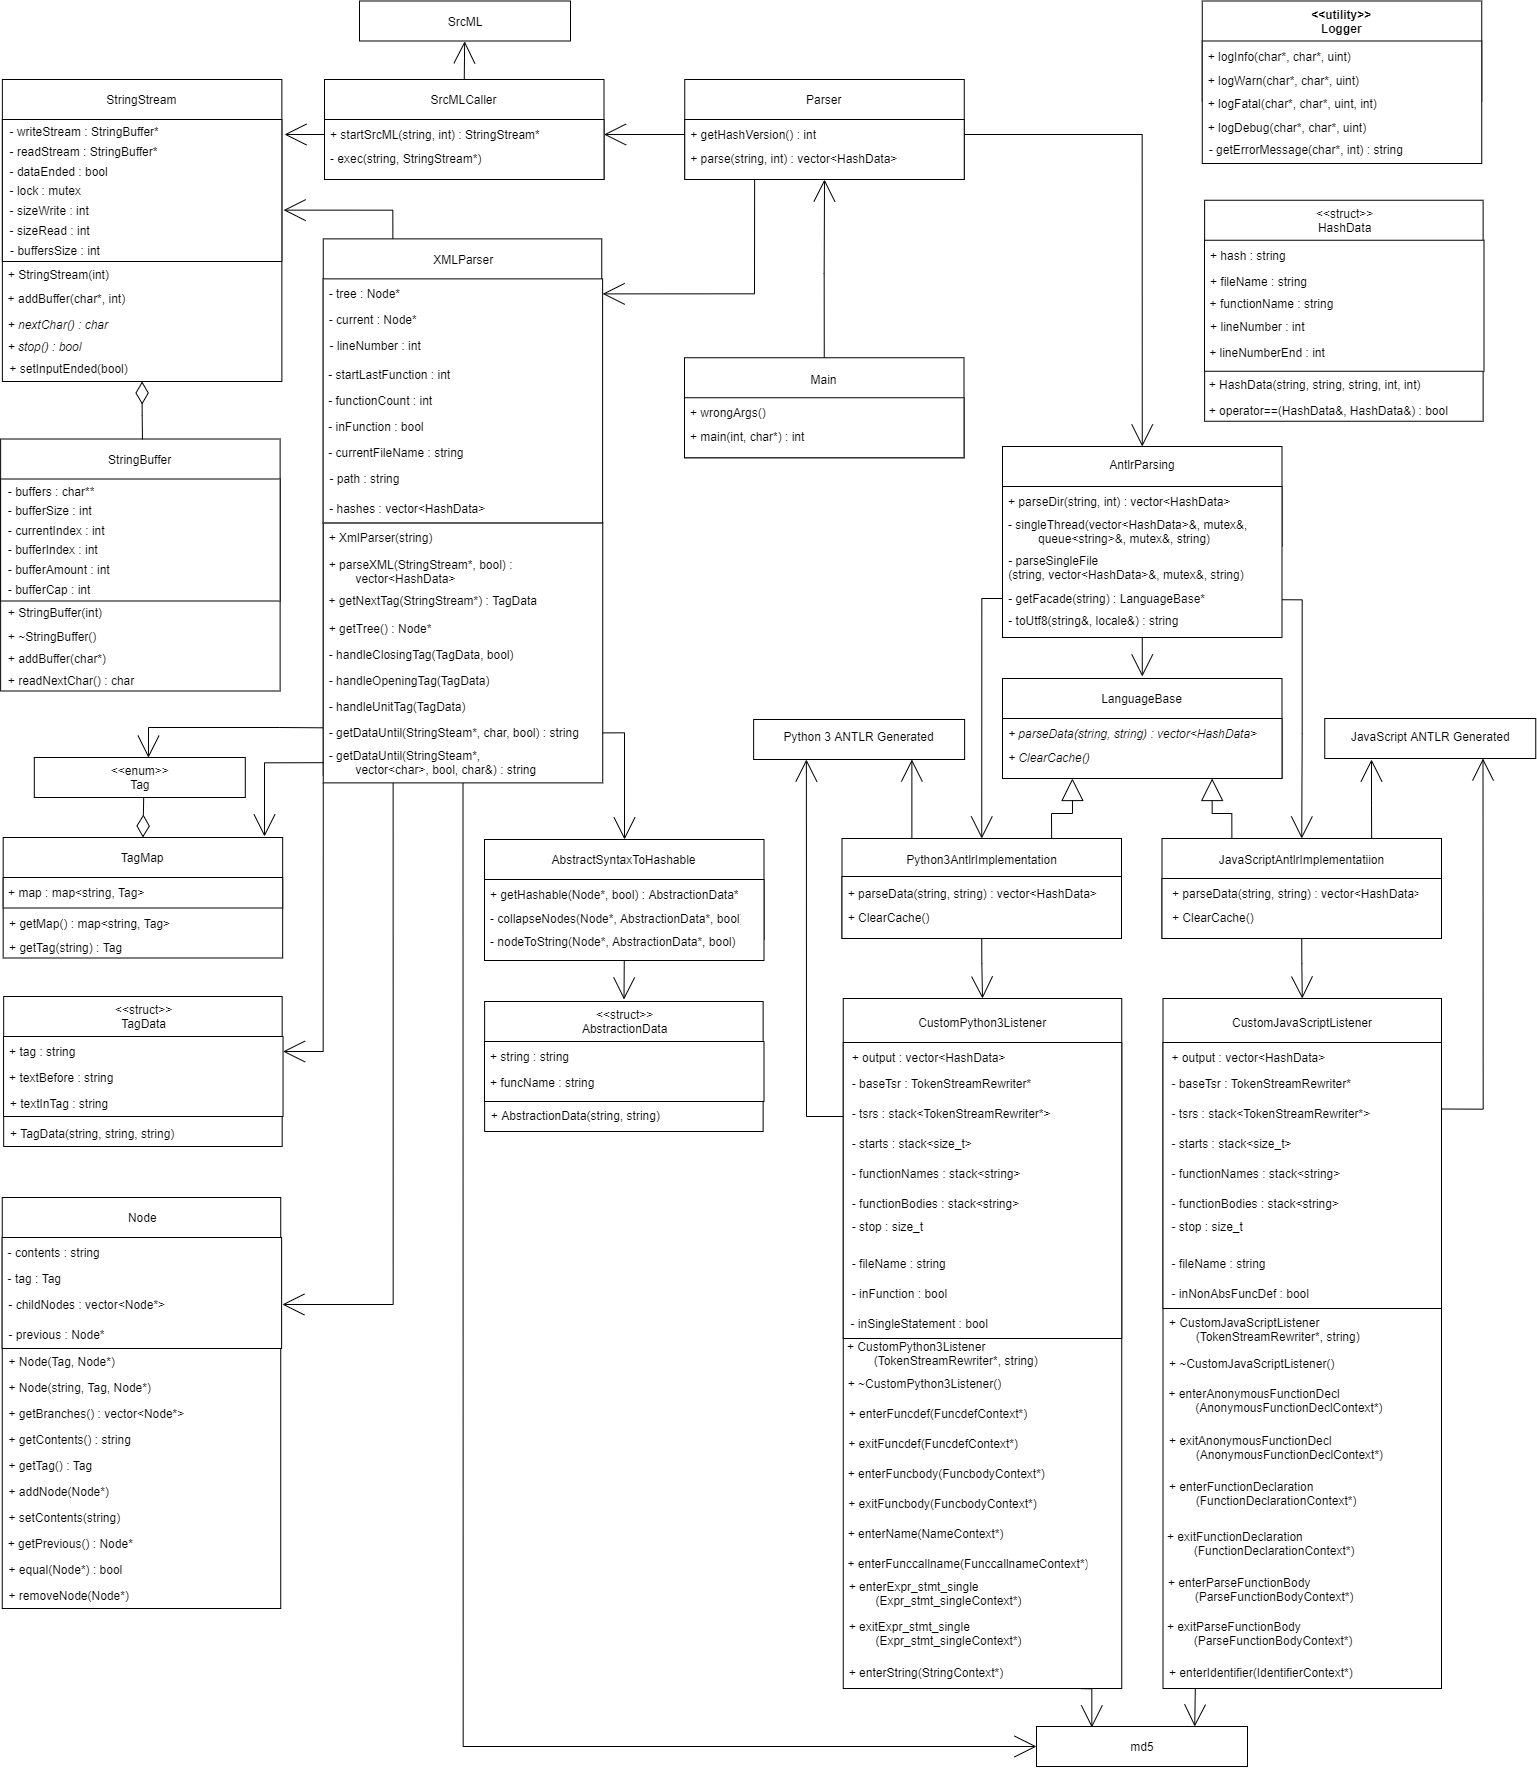
\includegraphics[width = \linewidth]{ParserUML.png}
    \caption{Parser UML class diagram}
    \label{fig:umlparser}
\end{figure}

\begin{figure}
    \centering
    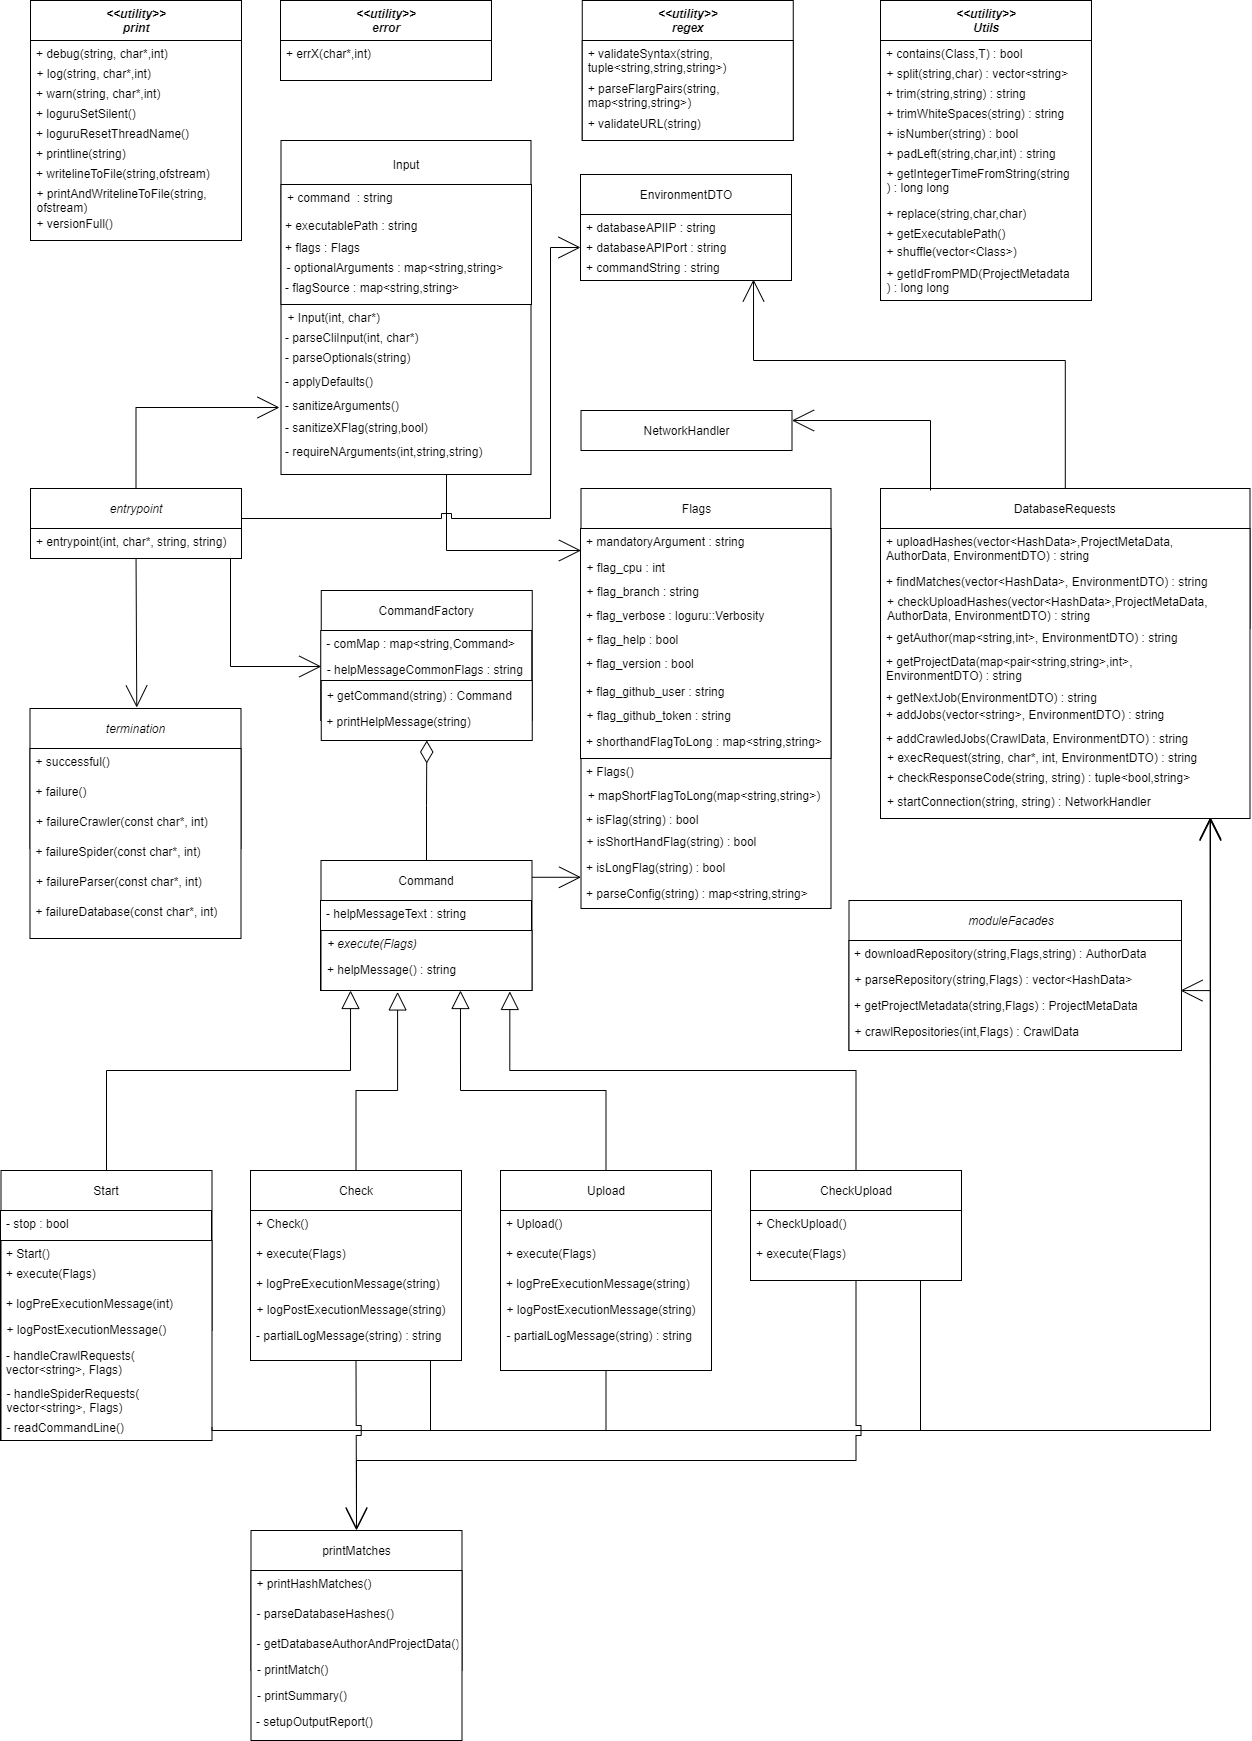
\includegraphics[width = \linewidth]{ControllerUML.png}
    \caption{Controller UML class diagram}
    \label{fig:umlcontroller}
\end{figure}

\begin{figure}
    \centering
    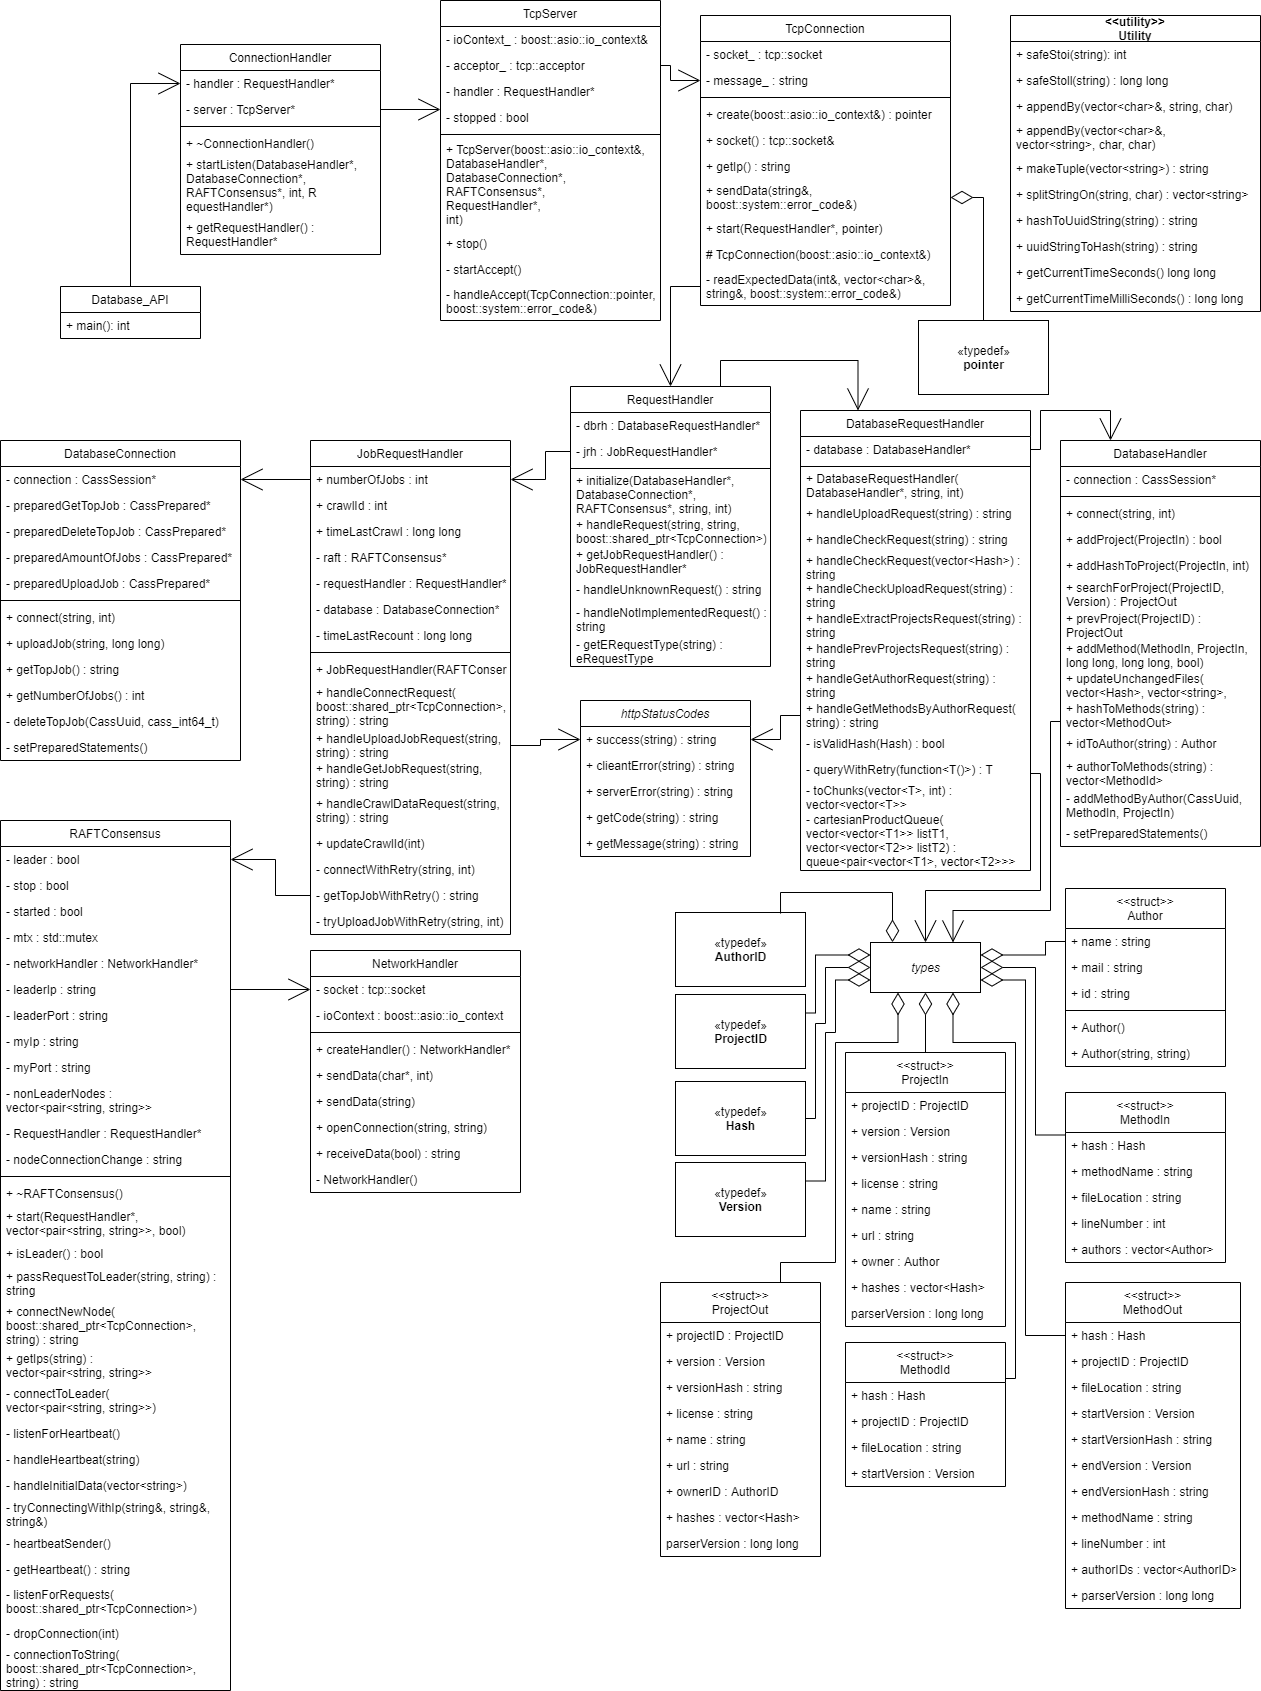
\includegraphics[width = \linewidth]{DatabaseAPIUML.png}
    \caption{Database API UML class diagram}
    \label{fig:umldatabase}
\end{figure}

\end{document}
